
\section{Introduction}

\subsection{Task}

\subsection{Datasets}

\subsubsection{ZIP}

\begin{figure}
 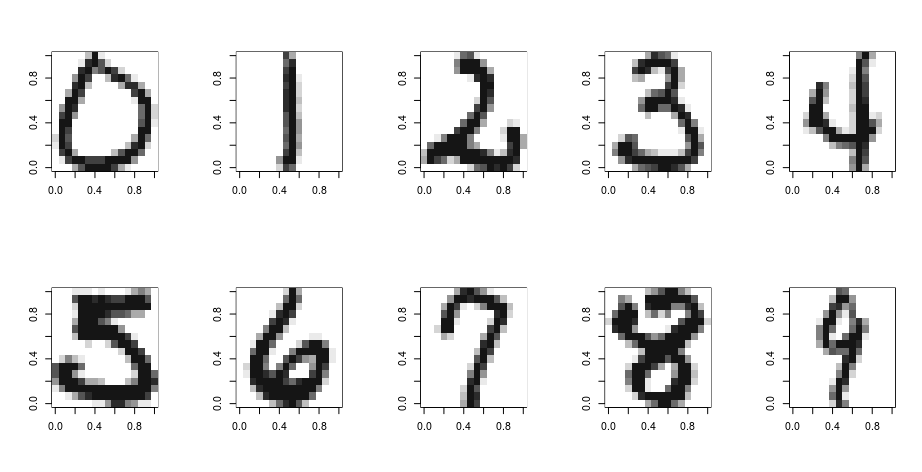
\includegraphics[width=\textwidth]{../plots/zip_dataset}
 \caption{Example images of the 10 classes of the ZIP dataset.}
\end{figure}

\subsubsection{MNIST}

\begin{figure}
 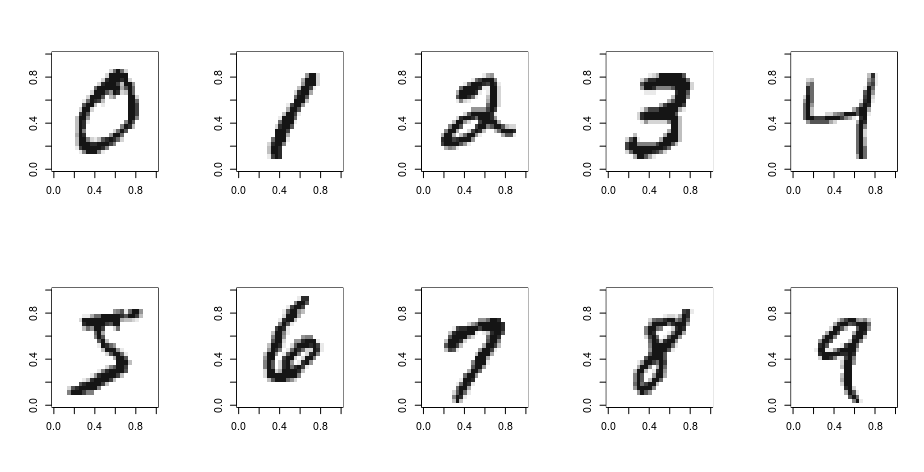
\includegraphics[width=\textwidth]{../plots/mnist_dataset}
 \caption{Example images of the 10 classes of the MNIST dataset.}
\end{figure}

\subsubsection{CIFAR10}

\begin{figure}
 \begin{minipage}{0.19\textwidth}
  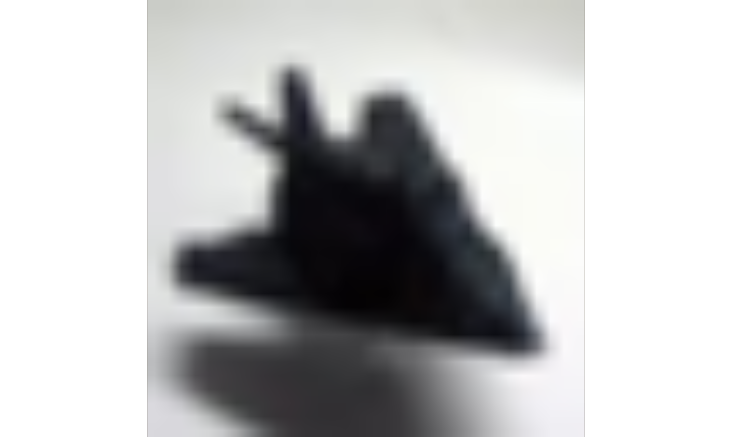
\includegraphics[width=1.5\textwidth]{../plots/cifar10-class0}
 \end{minipage}
 \begin{minipage}{0.19\textwidth}
  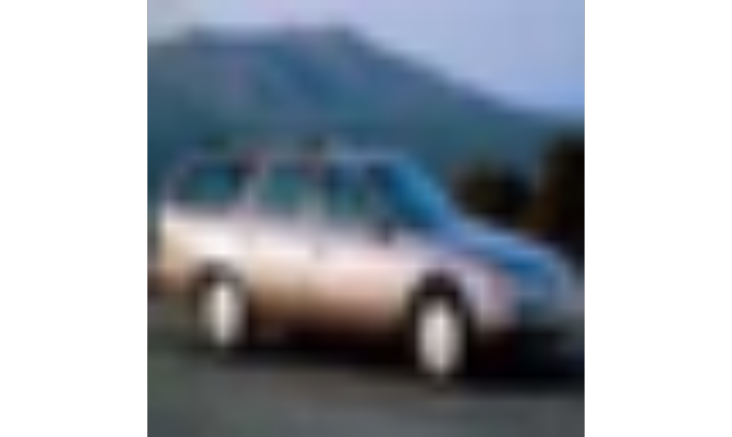
\includegraphics[width=1.5\textwidth]{../plots/cifar10-class1}
 \end{minipage}
 \begin{minipage}{0.19\textwidth}
  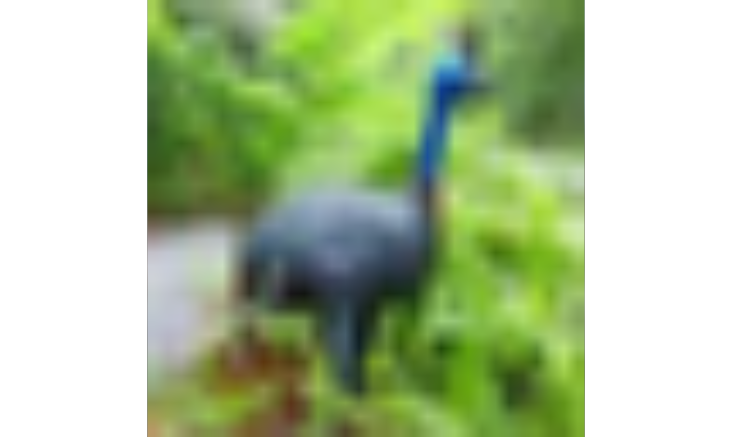
\includegraphics[width=1.5\textwidth]{../plots/cifar10-class2}
 \end{minipage}
 \begin{minipage}{0.19\textwidth}
  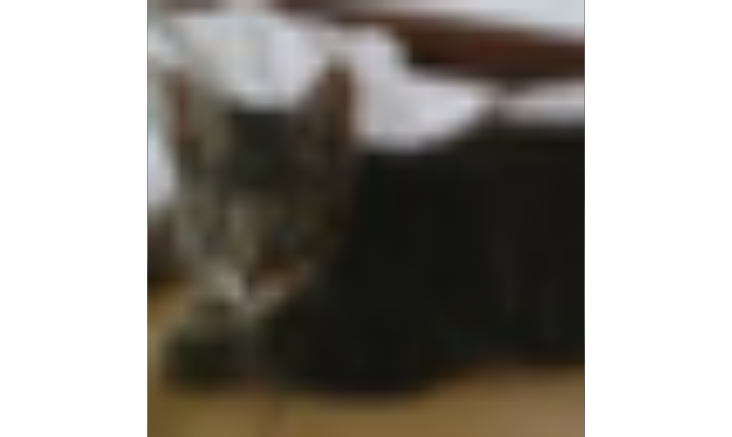
\includegraphics[width=1.5\textwidth]{../plots/cifar10-class3}
 \end{minipage}
 \begin{minipage}{0.19\textwidth}
  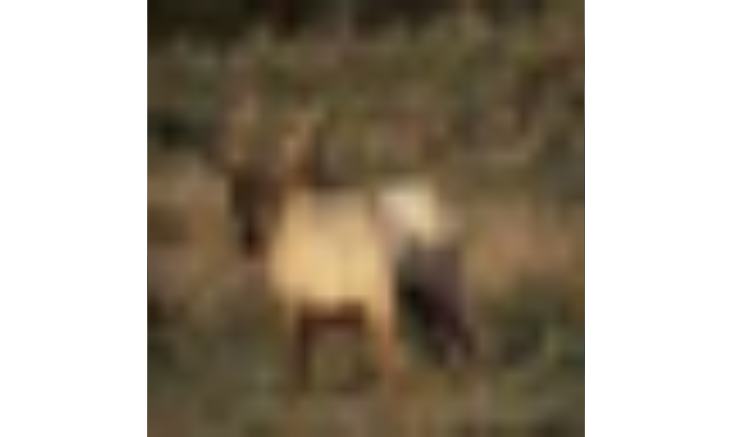
\includegraphics[width=1.5\textwidth]{../plots/cifar10-class4}
 \end{minipage}
 \begin{minipage}{0.19\textwidth}
  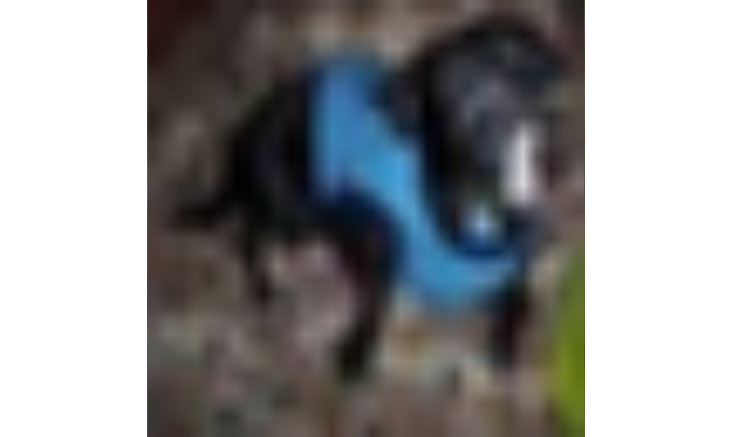
\includegraphics[width=1.5\textwidth]{../plots/cifar10-class5}
 \end{minipage}
 \begin{minipage}{0.19\textwidth}
  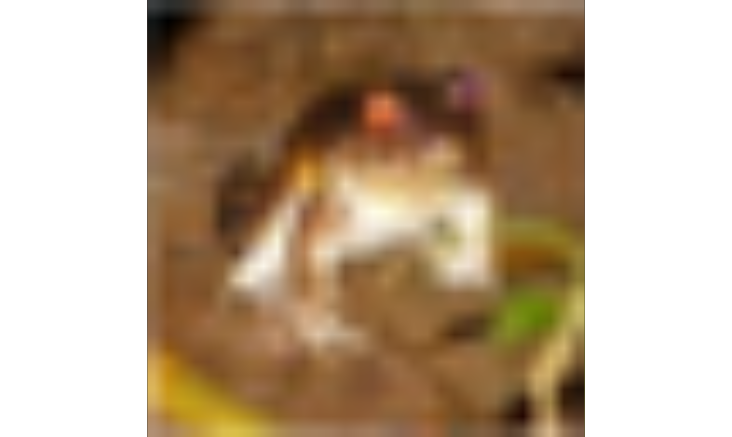
\includegraphics[width=1.5\textwidth]{../plots/cifar10-class6}
 \end{minipage}
 \begin{minipage}{0.19\textwidth}
  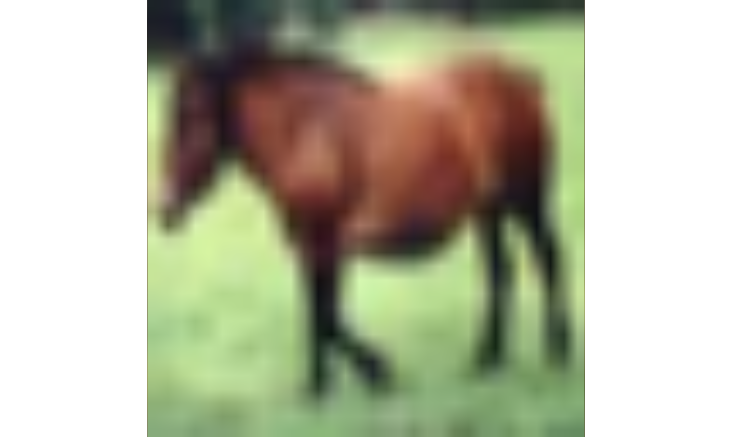
\includegraphics[width=1.5\textwidth]{../plots/cifar10-class7}
 \end{minipage}
 \begin{minipage}{0.19\textwidth}
  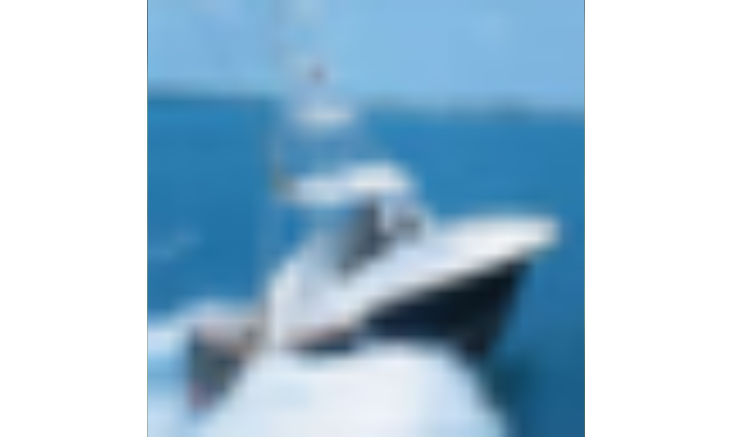
\includegraphics[width=1.5\textwidth]{../plots/cifar10-class8}
 \end{minipage}
 \begin{minipage}{0.19\textwidth}
  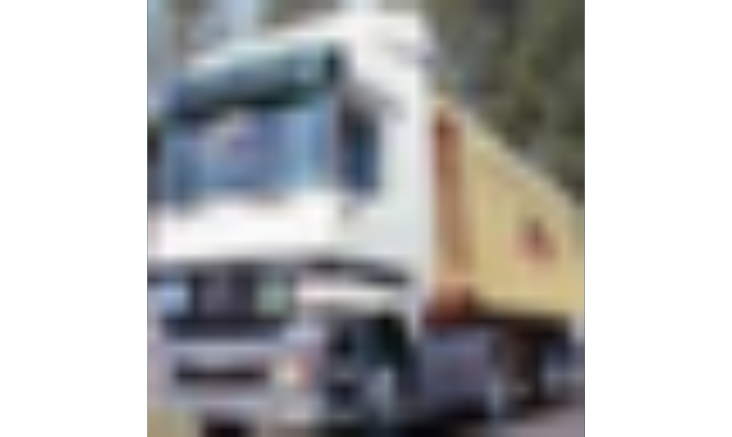
\includegraphics[width=1.5\textwidth]{../plots/cifar10-class9}
 \end{minipage}
 \caption{Example images for the 10 classes of the CIFAR10 dataset.}
\end{figure}
